\section{1174087 - Ilham Muhammad Ariq}
\subsection{Teori}
\begin{enumerate}
\item Jelaskan kenapa file teks harus di lakukan tokenizer. dilengkapi dengan ilustrasi atau gambar. 
	\hfill \break	
	Untuk memudahkan mesin memahami maksud dari apa yang kita inginkan dalam machine learning, kata pada teks disebut token, dan proses vektorisasi dari bentuk kata ke dalam token tersebut disebut tokenizer dan tokenizer akan merubah sebuah teks menjadi simbol, kata, ataupun biner dan bentuk lainnya kedalam token. Ilutrasinya misalkan saya mempunyai sebuah kalimat yaitu ”Nama Saya Ilham Muhammad Ariq” maka ketika kita lakukan proses tokenizer maka akan berubah menjadi ['Nama', 'Saya', 'Ilham','Muhammad','Ariq'].

	\item Jelaskan konsep dasar K Fold Cross Validation pada dataset komentar Youtube pada kode listing \ref{lst:7.0}.dilengkapi dengan ilustrasi atau gambar.
	\hfill \break
	\begin{lstlisting}[caption=K Fold Cross Validation,label={lst:7.0}]
		kfold = StratifiedKFold(n_splits=5)
		splits = kfold.split(d, d['CLASS'])
	\end{lstlisting}
	Pada koding diatas terdapat variabel kfold yang didalamnya berisi parameter split yang diisikan nilai 5. hal tersebut dimaksudkan untuk membuat pengolahan data akan diulang setiap datanya sebanyak lima kali dengan atribut class sebagai acuan pengolahan datanya. Lalu kemudian akan di hasilkan akurasi dari pengulangan data tersebut sebesar sekian persen tergantung datanya
	\begin{figure}[H]
    	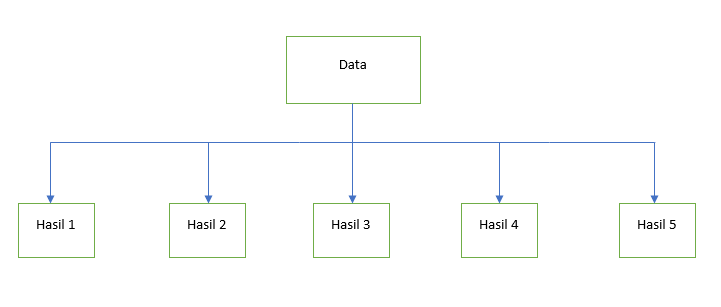
\includegraphics[width=4cm]{figures/1174087/7/1.png}
    	\centering
    	\caption{Illustrasi K Fold Cross Validation}
	\end{figure}
	\item Jelaskan apa maksudnya kode program \emph{for train, test in splits}.dilengkapi dengan ilustrasi atau gambar.
	\hfill \break
	Maksudnya yaitu untuk menguji apakah setiap data pada dataset sudah di split dan tidak terjadi penumpukan. Yang dimana maksudnya disetiap class tidak akan muncul id yang sama. Ilustrasinya misalkan kita memiliki 5 sepatu dengan model yang berbeda. Kemudian kita bagikan ke kedua orang , tentunya setiap orang yang menerima sepatu tidak memiliki model sepatu yang sama.

	\item Jelaskan apa maksudnya kode program \emph{train\_content = d['CONTENT'].iloc[train\_idx]} dan \emph{test\_content = d['CONTENT'].iloc[test\_idx]}. dilengkapi dengan ilustrasi atau gambar.
	\hfill \break
	Maksudnya yaitu mengambil data pada kolom atau index CONTENT yang merupakan bagian dari train idx dan test idx. Ilustrasinya, ketika data telah diubah menjadi train dan test maka kita dapat memilihnya untuk ditampilkan pada kolom yang diinginkan.

	\item Jelaskan apa maksud dari fungsi \emph{tokenizer = Tokenizer(num\_words=2000)} dan \emph{tokenizer.fit\_on\_texts(train\_content)}, dilengkapi dengan ilustrasi atau gambar.
		\begin{itemize}
			\item tokenizer = Tokennizer(num\_words=2000) digunakan untuk membaca kalimat yang telah dibuat menjadi token sebanyak 2000 kata
    		\item fit\_on\_texts digunakan untuk membuat membaca data token teks yang telah dimasukan kedalam fungsi yaitu fungsi train\_konten
		\end{itemize}
	\begin{figure}[H]
		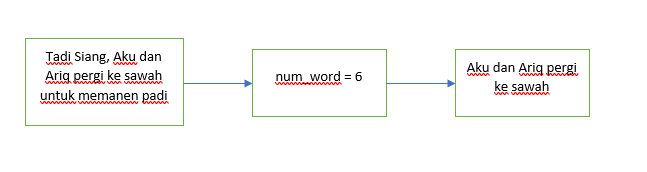
\includegraphics[width=4cm]{figures/1174087/7/2.png}
		\centering
		\caption{Illustrasi fit tokenizer dan num\_word=2000}
	\end{figure}
	
	\item Jelaskan apa maksud dari fungsi \emph{d\_train\_inputs = tokenizer.texts\_to\_matrix(train\_content, mode='tfidf')} dan \emph{d\_test\_inputs = tokenizer.texts\_to\_matrix(test\_content, mode='tfidf')}, dilengkapi dengan ilustrasi kode dan atau gambar.
	\hfill \break
	Untuk digunakan sebagai pengubah urutan teks yang tadi telah dilakukan tkoenizer menjadi matriks yang berurutan seperti tf idf
	\begin{figure}[H]
		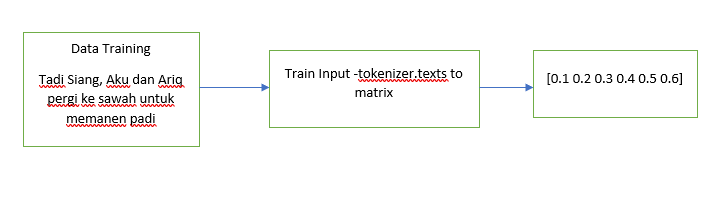
\includegraphics[width=4cm]{figures/1174087/7/3.png}
		\centering
		\caption{Illustrasi d train inputs = tokenizer.texts to matrix}
	\end{figure}
	
	\item Jelaskan apa maksud dari fungsi \emph{d\_train\_inputs = d\_train\_inputs/np.amax(np.absolute(d\_train\_inputs))} dan \emph{d\_test\_inputs = d\_test\_inputs/np.amax(np.absolute(d\_test\_inputs))}, dilengkapi dengan ilustrasi atau gambar.
	\hfill \break
	Fungsi tersebut digunakan untuk membagi matriks tfidf dnegan penentuan maksimum array sepanjang sumbu sehingga akan menimbulkan garis ke bawah dan ke atas yang membentuk gambar v. Lalu hasil tersebut akan dimasukkan ke variabel d train input dan d test input dengan methode absolute. Yang berarti tanpa bilangan negatif.
	
	\item Jelaskan apa maksud fungsi dari \emph{d\_train\_outputs = np\_utils.to\_categorical(d['CLASS'].iloc[train\_idx])} dan \emph{d\_test\_outputs = np\_utils.to\_categorical(d['CLASS'].iloc[test\_idx])} dalam kode program, dilengkapi dengan ilustrasi atau gambar.
	\hfill \break
	Maksud dari fungsi tersebut yaitu untuk merubah nilai vektor yang ada pada atribut class menjadi bentuk matrix dengan pengurutan berdasarkan data index training dan testing.
	
	\item Jelaskan apa maksud dari fungsi di listing \ref{lst:7.1}. Gambarkan ilustrasi Neural Network nya dari model kode tersebut.
	\hfill \break
	\begin{lstlisting}[caption=Membuat model Neural Network,label={lst:7.1}]
		   model = Sequential()
		   model.add(Dense(512, input_shape=(2000,)))
		   model.add(Activation('relu'))
		   model.add(Dropout(0.5))
		   model.add(Dense(2))
		   model.add(Activation('softmax'))
	\end{lstlisting}
	\hfill \break
	Penjelasannya sebagai berikut:	
	\begin{itemize}
	\item Melakukan pemodelan Sequential
	\item Layer pertama dense dari 512 neuron untuk inputan dengan inputan tadi yang sudah dijadikan matriks sebanyak 2000
	\item Activationnya menggunakan fungsi relu yaitu jika ada inputan dengan nilai maksimum maka inputan itu yang akan terpilih.
	\item Dropout ini untuk melakukan pembobotan,dimana pembobotan hanya dilakukan 50 persen saja agar tidak terjadi penumpukan data dari dense inputan tadi
	\item Dense 2 mengkategorikan 2 neuron untuk output nya yaitu 1 dan 0.
	\item Untuk dense diatas aktivasinya menggunakan fungsi Softmax. 
	\end{itemize}
	
	\begin{figure}[H]
		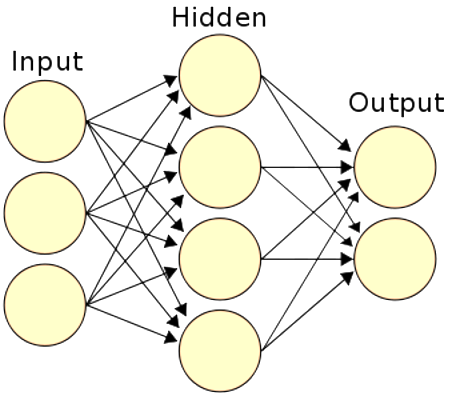
\includegraphics[width=4cm]{figures/1174087/7/4.png}
		\centering
		\caption{Illustrasi Neural Network Pemodelan}
	\end{figure}
	
	\item Jelaskan apa maksud dari fungsi di listing \ref{lst:7.2} dengan parameter tersebut.
	\hfill \break
	\begin{lstlisting}[caption=Compile model,label={lst:7.2}]
		model.compile(loss='categorical_crossentropy', optimizer='adamax',
						  metrics=['accuracy'])
	\end{lstlisting}
	Melakukan peng compile-an dari model Sequential tadi dengan Loss yandengang merupakanfungsioptimisasiskormenggunakancategorical crossentropy,danmenggunakan algoritma adam sebagai optimizer. Adam yaitu algoritma pengoptimalan yangdapatdigunakansebagaigantidariprosedurpenurunangradienstokastikklasik untuk memperbarui bobot jaringan yang berulang berdasarkan data training.Dengan metrik yaitu fungsi yang digunakan untuk menilai kinerja mode Anda disini menggunakan fungsi accuracy. 
	
	\item Jelaskan apa itu Deep Learning
	\hfill \break
	Deep Learning adalah subbidang machine learning yang berkaitan dengan algoritma yang terinspirasi oleh struktur dan fungsi otak yang disebut jaringan saraf tiruan atau Artificial Neural Networks. Jaringan saraf tiruan, algoritma yang terinspirasi oleh otak manusia, belajar dari sejumlah besar data. Demikian pula dengan bagaimana kita belajar dari pengalaman, algoritma pembelajaran yang mendalam akan melakukan tugas berulang kali,setiap kali sedikit mengubahnya untuk meningkatkan hasilnya.
	 
	\item Jelaskan apa itu Deep Neural Network, dan apa bedanya dengan Deep Learning
	\hfill \break
	Deep Neural Network adalah jaringan syaraf tiruan (JST) dengan beberapa lapisan antara lapisan input dan output. DNN menemukan manipulasi matematis yang benar untuk mengubah input menjadi output, apakah itu hubungan linear atau hubungan non-linear. Merupakan jaringan syaraf dengan tingkat kompleksitas tertentu, jaringan syaraf dengan lebih dari dua lapisan. Deep Neural Network menggunakan pemodelan matematika yang canggih untuk memproses data dengan cara yang kompleks. 
   \hfill \break	
	DNN hanya terdiri dari dua laipsan yaitu input dan output, sedangkan dalam Deep learning kita dapat mendefiniskan layer sebanyak yang kita inginkan atau butuhkan.
	
	\item Jelaskan dengan ilustrasi gambar buatan sendiri(langkah per langkah) bagaimana perhitungan algoritma konvolusi dengan ukuran stride (NPM mod3+1) x (NPM mod3+1) yang terdapat max pooling.(nilai 30)
	\hfill \break
	Sebelum membuat ilustrasi perlu di ketahui apa itu stride, stride adalah acuan atau parameter yang menentukan pergeseran pada filter fixcel. sebagai contoh nilai stride 1 yang berarti filter akan bergeser sebanyak satu fixcel secara vertikal dan horizontal. selanjutnya apa itu max pooling contoh pada suatu gambar di tentukan Max Pooling dari 3 x 3 dengan stride 1 yang berarti setiap pergeseran 1 pixcel akan diambil nilai terbesar dari pixcel 3 x 3 tersebut.
	\begin{figure}[H]
		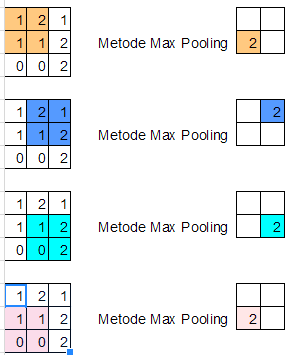
\includegraphics[width=4cm]{figures/1174087/7/5.png}
		\centering
		\caption{Illustrasi perhitungan stride 1 max pooling}
	\end{figure}
\end{enumerate}
\subsection{Praktek}
\begin{enumerate}
\item Jelaskan kode program pada blok \# In[1]. Jelaskan arti dari setiap baris kode yang dibuat(harus beda dengan teman sekelas) dan hasil luarannya dari komputer sendiri.
\lstinputlisting[firstline=8, lastline=14]{src/1174087/7/1174087.py}

\item Jelaskan kode program pada blok \# In[2]. Jelaskan arti dari setiap baris kode yang dibuat(harus beda dengan teman sekelas) dan hasil luarannya dari komputer sendiri.
\lstinputlisting[firstline=16, lastline=39]{src/1174087/7/1174087.py}

\item Jelaskan kode program pada blok \# In[3]. Jelaskan arti dari setiap baris kode yang dibuat(harus beda dengan teman sekelas) dan hasil luarannya dari komputer sendiri.
\lstinputlisting[firstline=41, lastline=51]{src/1174087/7/1174087.py}

\item Jelaskan kode program pada blok \# In[4]. Jelaskan arti dari setiap baris kode yang dibuat(harus beda dengan teman sekelas) dan hasil luarannya dari komputer sendiri.
\lstinputlisting[firstline=53, lastline=63]{src/1174087/7/1174087.py}

\item Jelaskan kode program pada blok \# In[5]. Jelaskan arti dari setiap baris kode yang dibuat(harus beda dengan teman sekelas) dan hasil luarannya dari komputer sendiri.
\lstinputlisting[firstline=65, lastline=69]{src/1174087/7/1174087.py}

\item Jelaskan kode program pada blok \# In[6]. Jelaskan arti dari setiap baris kode yang dibuat(harus beda dengan teman sekelas) dan hasil luarannya dari komputer sendiri.
\lstinputlisting[firstline=71, lastline=76]{src/1174087/7/1174087.py}

\item Jelaskan kode program pada blok \# In[7]. Jelaskan arti dari setiap baris kode yang dibuat(harus beda dengan teman sekelas) dan hasil luarannya dari komputer sendiri.
\lstinputlisting[firstline=78, lastline=84]{src/1174087/7/1174087.py}

\item Jelaskan kode program pada blok \# In[8]. Jelaskan arti dari setiap baris kode yang dibuat(harus beda dengan teman sekelas) dan hasil luarannya dari komputer sendiri.
\lstinputlisting[firstline=86, lastline=98]{src/1174087/7/1174087.py}

\item Jelaskan kode program pada blok \# In[9]. Jelaskan arti dari setiap baris kode yang dibuat(harus beda dengan teman sekelas) dan hasil luarannya dari komputer sendiri.
\lstinputlisting[firstline=100, lastline=107]{src/1174087/7/1174087.py}

\item Jelaskan kode program pada blok \# In[10]. Jelaskan arti dari setiap baris kode yang dibuat(harus beda dengan teman sekelas) dan hasil luarannya dari komputer sendiri.
\lstinputlisting[firstline=108, lastline=132]{src/1174087/7/1174087.py}

\item Jelaskan kode program pada blok \# In[11]. Jelaskan arti dari setiap baris kode yang dibuat(harus beda dengan teman sekelas) dan hasil luarannya dari komputer sendiri.
\lstinputlisting[firstline=134, lastline=138]{src/1174087/7/1174087.py}

\item Jelaskan kode program pada blok \# In[12]. Jelaskan arti dari setiap baris kode yang dibuat(harus beda dengan teman sekelas) dan hasil luarannya dari komputer sendiri.
\lstinputlisting[firstline=140, lastline=152]{src/1174087/7/1174087.py}

\item Jelaskan kode program pada blok \# In[13]. Jelaskan arti dari setiap baris kode yang dibuat(harus beda dengan teman sekelas) dan hasil luarannya dari komputer sendiri.
\lstinputlisting[firstline=154, lastline=209]{src/1174087/7/1174087.py}

\item Jelaskan kode program pada blok \# In[14]. Jelaskan arti dari setiap baris kode yang dibuat(harus beda dengan teman sekelas) dan hasil luarannya dari komputer sendiri.
\lstinputlisting[firstline=211, lastline=233]{src/1174087/7/1174087.py}

\item Jelaskan kode program pada blok \# In[15]. Jelaskan arti dari setiap baris kode yang dibuat(harus beda dengan teman sekelas) dan hasil luarannya dari komputer sendiri.
\lstinputlisting[firstline=235, lastline=241]{src/1174087/7/1174087.py}

\item Jelaskan kode program pada blok \# In[16]. Jelaskan arti dari setiap baris kode yang dibuat(harus beda dengan teman sekelas) dan hasil luarannya dari komputer sendiri.
\lstinputlisting[firstline=243, lastline=245]{src/1174087/7/1174087.py}

\item Jelaskan kode program pada blok \# In[17]. Jelaskan arti dari setiap baris kode yang dibuat(harus beda dengan teman sekelas) dan hasil luarannya dari komputer sendiri.
\lstinputlisting[firstline=247, lastline=249]{src/1174087/7/1174087.py}

\item Jelaskan kode program pada blok \# In[18]. Jelaskan arti dari setiap baris kode yang dibuat(harus beda dengan teman sekelas) dan hasil luarannya dari komputer sendiri.
\lstinputlisting[firstline=251, lastline=258]{src/1174087/7/1174087.py}

\item Jelaskan kode program pada blok \# In[19]. Jelaskan arti dari setiap baris kode yang dibuat(harus beda dengan teman sekelas) dan hasil luarannya dari komputer sendiri.
\lstinputlisting[firstline=260, lastline=280]{src/1174087/7/1174087.py}

\item Jelaskan kode program pada blok \# In[20]. Jelaskan arti dari setiap baris kode yang dibuat(harus beda dengan teman sekelas) dan hasil luarannya dari komputer sendiri.
\lstinputlisting[firstline=282, lastline=288]{src/1174087/7/1174087.py}
\end{enumerate}
\subsection{Penanganan Error}
\begin{enumerate}
	\item SS Error
	\begin{figure}[H]
		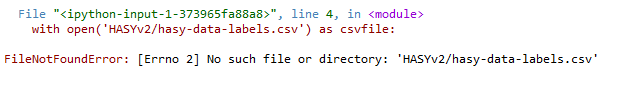
\includegraphics[width=4cm]{figures/1174087/7/error.png}
		\centering
		\caption{File Not Found error}
	\end{figure}
	\item Jenis Error
	\begin{itemize}
		\item File Not Found Error
	\end{itemize}
	\item Cara Penanganan
	\hfill\break
	Dengan cara menyesuaikan letak file yang ingin dibaca/ digunakan
\end{enumerate}
\subsection{Bukti Tidak Plagiat}
\begin{figure}[H]
    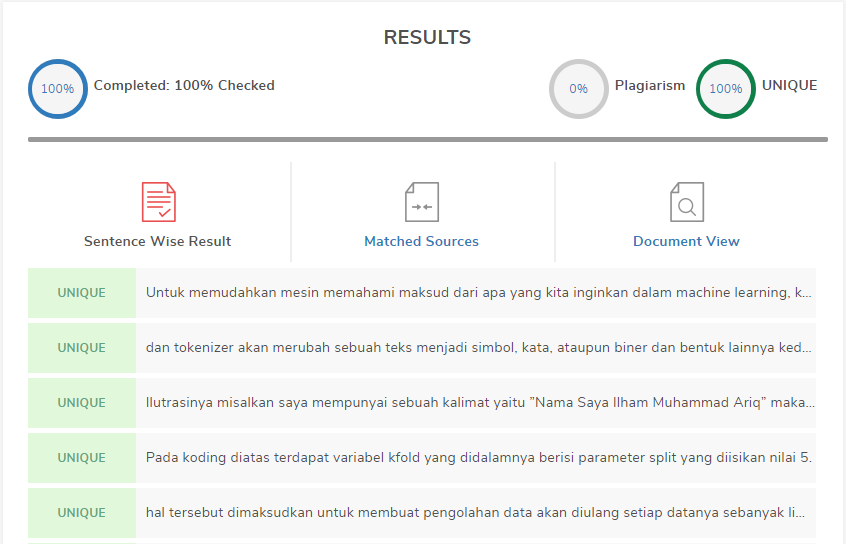
\includegraphics[width=4cm]{figures/1174087/7/plagiat.png}
    \centering
    \caption{Tidak Melakukan Plagiat Pada Ch 7}
\end{figure}

\subsection{Link Video Youtube}
https://youtu.be/XPdKuIEMeu8